\documentclass[man,floatsintext]{apa6}
\usepackage{lmodern}
\usepackage{amssymb,amsmath}
\usepackage{ifxetex,ifluatex}
\usepackage{fixltx2e} % provides \textsubscript
\ifnum 0\ifxetex 1\fi\ifluatex 1\fi=0 % if pdftex
  \usepackage[T1]{fontenc}
  \usepackage[utf8]{inputenc}
\else % if luatex or xelatex
  \ifxetex
    \usepackage{mathspec}
  \else
    \usepackage{fontspec}
  \fi
  \defaultfontfeatures{Ligatures=TeX,Scale=MatchLowercase}
\fi
% use upquote if available, for straight quotes in verbatim environments
\IfFileExists{upquote.sty}{\usepackage{upquote}}{}
% use microtype if available
\IfFileExists{microtype.sty}{%
\usepackage{microtype}
\UseMicrotypeSet[protrusion]{basicmath} % disable protrusion for tt fonts
}{}
\usepackage{hyperref}
\hypersetup{unicode=true,
            pdftitle={Who Needs Privacy?},
            pdfauthor={Tobias Dienlin~\& Miriam Metzger},
            pdfkeywords={Privacy, need for privacy, personality, anonymity, integrity, SEM},
            pdfborder={0 0 0},
            breaklinks=true}
\urlstyle{same}  % don't use monospace font for urls
\usepackage{graphicx,grffile}
\makeatletter
\def\maxwidth{\ifdim\Gin@nat@width>\linewidth\linewidth\else\Gin@nat@width\fi}
\def\maxheight{\ifdim\Gin@nat@height>\textheight\textheight\else\Gin@nat@height\fi}
\makeatother
% Scale images if necessary, so that they will not overflow the page
% margins by default, and it is still possible to overwrite the defaults
% using explicit options in \includegraphics[width, height, ...]{}
\setkeys{Gin}{width=\maxwidth,height=\maxheight,keepaspectratio}
\IfFileExists{parskip.sty}{%
\usepackage{parskip}
}{% else
\setlength{\parindent}{0pt}
\setlength{\parskip}{6pt plus 2pt minus 1pt}
}
\setlength{\emergencystretch}{3em}  % prevent overfull lines
\providecommand{\tightlist}{%
  \setlength{\itemsep}{0pt}\setlength{\parskip}{0pt}}
\setcounter{secnumdepth}{0}
% Redefines (sub)paragraphs to behave more like sections
\ifx\paragraph\undefined\else
\let\oldparagraph\paragraph
\renewcommand{\paragraph}[1]{\oldparagraph{#1}\mbox{}}
\fi
\ifx\subparagraph\undefined\else
\let\oldsubparagraph\subparagraph
\renewcommand{\subparagraph}[1]{\oldsubparagraph{#1}\mbox{}}
\fi

%%% Use protect on footnotes to avoid problems with footnotes in titles
\let\rmarkdownfootnote\footnote%
\def\footnote{\protect\rmarkdownfootnote}


  \title{Who Needs Privacy?}
    \author{Tobias Dienlin\textsuperscript{1}~\& Miriam Metzger\textsuperscript{2}}
    \date{}
  
\shorttitle{Who Needs Privacy?}
\affiliation{
\vspace{0.5cm}
\textsuperscript{1} University of Hohenheim\\\textsuperscript{2} University of California, Santa Barbara}
\keywords{Privacy, need for privacy, personality, anonymity, integrity, SEM}
\usepackage{csquotes}
\usepackage{upgreek}
\captionsetup{font=singlespacing,justification=justified}

\usepackage{longtable}
\usepackage{lscape}
\usepackage{multirow}
\usepackage{tabularx}
\usepackage[flushleft]{threeparttable}
\usepackage{threeparttablex}

\newenvironment{lltable}{\begin{landscape}\begin{center}\begin{ThreePartTable}}{\end{ThreePartTable}\end{center}\end{landscape}}

\makeatletter
\newcommand\LastLTentrywidth{1em}
\newlength\longtablewidth
\setlength{\longtablewidth}{1in}
\newcommand{\getlongtablewidth}{\begingroup \ifcsname LT@\roman{LT@tables}\endcsname \global\longtablewidth=0pt \renewcommand{\LT@entry}[2]{\global\advance\longtablewidth by ##2\relax\gdef\LastLTentrywidth{##2}}\@nameuse{LT@\roman{LT@tables}} \fi \endgroup}


\usepackage{lineno}

\linenumbers
\setlength{\parskip}{0em}
\raggedbottom

\authornote{Tobias Dienlin, Department of Media Psychology, University of Hohenheim, Germany; Miriam Metzger, Department of Communication, University of California, Santa Barbara, United States of America.

Correspondence concerning this article should be addressed to Tobias Dienlin, University of Hohenheim, Department of Media Psychology (540F), 70599 Stuttgart, Germany. E-mail: \href{mailto:tobias.dienlin@uni-hohenheim.de}{\nolinkurl{tobias.dienlin@uni-hohenheim.de}}}

\abstract{
This study analyzes how personality traits relate to need for privacy. We focus on three dimensions: (a) need for privacy from government surveillance, (b) need for privacy from other individuals, and (c) need for anonymity. Using an online questionnaire with 271 student respondents, several significant relationships were found. For example, results showed that less sociable people desired considerably more privacy on all three dimensions. Somewhat more controversially, people who reported less integrity also desired noticeably more anonymity. While anxious people desired slightly less privacy from government surveillance, risk avoidant people desired considerably more privacy from other people. Traditionalism did not relate to need for privacy. Together, the results have several implications. For example, they shed some light on the nothing-to-hide argument: A person who desires more anonymity might indeed be of less integrity. However, it is equally plausible that this person is just a little less sociable.

}

\begin{document}
\maketitle

In light of the increasing digitization of everyday life, which has led to several sweeping societal changes such as the commodification and monetization of personal information (Sevignani, 2016), privacy has become a major topic of interest. Despite its importance, however, we still know surprisingly little about the relation between privacy and personality (e.g., Masur, 2018, p. 155). Why do some people need more privacy than others, and how do these people differ from one another? We think that a better understanding of the relation between personality and privacy is crucial: Several theories argue that personality determines privacy behaviors (e.g., Masur, 2018), however, to date there is almost no empirical research that can be used to deduct well-informed hypotheses. As a result, the main question of this paper is as follows: What are personality facets that can be used to best explain peoples' need for privacy?

\hypertarget{the-need-for-privacy}{%
\subsection{The Need for Privacy}\label{the-need-for-privacy}}

Privacy as a theoretical concept is both complicated and contested (Nissenbaum, 2010, p. 71). Hence, we begin by outlining our own understanding of privacy. First and foremost, privacy captures the extent of voluntary withdrawal from others (Westin, 1967). Several models suggest that privacy is multi-dimensional. For example, in a theory-driven treatise Burgoon (1982) argued that privacy has four dimensions: informational, social, psychological, and physical privacy. Pedersen (1979), by contrast, did an empirical factor analysis (initially starting with 94 items) and suggested that privacy exists on six dimensions: reserve, isolation, solitude, intimacy with friends, intimacy with family, and anonymity. In addition, Schwartz (1968) differentiated between horizontal and vertical privacy; whereas horizontal privacy captures withdrawal from peers, vertical privacy addresses withdrawal from superiors or institutions (e.g., government agencies). Finally, one can also distinguish between the objective privacy context, the subjective privacy perception, the psychological need for privacy (which is both a situational and dispositional need), and the resulting privacy behavior (often represented by self-disclosure) (Dienlin, 2014).

For the purpose of this study, we combine the aforementioned notions and focus on (a) vertical privacy with regard to the need for withdrawal from government surveillance, (b) horizontal privacy in terms of the need for withdrawal from peers, friends, or acquaintances, and (c) both horizontal and vertical privacy as captured by the general need for anonymity.

In order to guide the selection of personality dimensions that might explain need for privacy best, it is useful to determine why people actually need privacy. Westin (1967) defined four primary positive purposes of privacy: (1) self-development (i.e., the integration of experiences into meaningful patterns), (2) autonomy (i.e., the desire to avoid being manipulated and dominated), (3) emotional release (i.e., the release of tension from social role demands), and (4) protected communication (i.e., the ability to foster intimate relationships). Not least, privacy facilitates self-disclosure (Dienlin, 2014), which is vital for attaining social support, initiating relationships, and getting close to one another (Omarzu, 2000).

On the other hand, however, too much privacy can also be problematic. Because human beings are inherently social, being overly cut-off from others can impede flourishing, nurture deviant behavior, or introduce power asymmetries (Altman, 1975). \enquote{{[}T{]}he feminist critique rightfully argued that for men, the private sphere can be a shielded sphere in which female suppression is not sanctioned.} (DeCew, 1997, p. 81, as cited by Masur, 2018, p.~38). Next, and as mentioned above, privacy fosters self-disclosure. However, any self-disclosure is also always a potential risk because others might disagree, disapprove, or misuse the information in other contexts (Petronio, 2010).

\hypertarget{predicting-the-need-for-privacy}{%
\subsection{Predicting the Need for Privacy}\label{predicting-the-need-for-privacy}}

In what follows we now explore several personality aspects that we think might predict the need for privacy. As there is no established theory that dovetails privacy and personality, it is difficult to deduct precise and well-informed hypotheses. The rationales that we outline below should hence considered to be tentative suggestions. Also, please note that we elaborate only on those dimensions of need for privacy for which plausible rationales could be found.

The general underlying theoretical framework that guided our selection process was the big five approach (e.g., John \& Srivastava, 1999). Note that privacy concerns, a variable conceptually close to need for privacy, shows only negligible relations with the big five factors (Bansal, Zahedi, \& Gefen, 2010; Junglas, Johnson, \& Spitzmüller, 2008). In order to be more precise, we hence follow the advice by Paunonen and Ashton (2001) and refer to specific personality facets instead of generic personality factors. To illustrate, instead of dwelling on the general factor of \emph{extraversion}, we instead focused on the facet \emph{gregariousness}, which we consider to be more pertinent.

Our reasoning was guided by another central theoretical thought. As implied above, privacy can be either positive or negative. Similarly, other people, the government, and anonymity can be considered either a \emph{resource} or a \emph{threat}. Having information about a person's personality can inform us whether he or she is more likely to think of others as a resource or a threat. It follows that if other people are considered a threat it seems to be more likely that a person will desire more privacy from others, and vice versa (Altman, 1976).

\hypertarget{sociability}{%
\subsubsection{Sociability}\label{sociability}}

First, we argue that need for privacy should be closely related to a person's sociability or gregariousness (which is a subdimension of extraversion, John \& Srivastava, 1999). Sociability captures whether people prefer to spend their time alone or with company. It seems plausible that people who are more sociable are also more likely to think of other people as a resource, which is why they should generally desire less interpersonal privacy and less anonymity (e.g., Buss, 2001). Put differently, given that privacy is a voluntary withdrawal from society (Westin, 1967), we expect that people who are less sociable, more reserved, or more shy should have a greater need for privacy from others.

This rationale is supported by several empirical studies: Extroverted people desire less privacy (Morton, 2013), people who describe themselves as introverted thinkers are more likely to prefer social isolation (Pedersen, 1982), and introverted people are more likely to report invasions of privacy (Stone, 1986).

\hypertarget{integrity}{%
\subsubsection{Integrity}\label{integrity}}

More controversially, it has been argued that people need privacy because they have something to hide. The so-called nothing-to-hide argument states that \enquote{If you have nothing to hide, you have nothing to fear.} As described by Solove, the nothing-to-hide argument says that data mining and surveillance by government entities \enquote{is not likely to be threatening to the privacy of law-abiding citizens. Only those who are engaged in illegal activities have a reason to hide this information} (Solove, 2007, p. 753). Hence, another potential predictor of why people need privacy could also be a so-called \enquote{lack of integrity}.

Because integrity is a delicate concept, let us first try to define it conceptually. Although in terms of a scientific definition there is no consensus, most scholars seem to agree that integrity \enquote{incorporates a tendency to comply with social norms, avoid deviant behavior, and embrace a sense of justice, truthfulness, and fairness} (Connelly, Lilienfeld, \& Schmeelk, 2006, p. 82). In order to sidestep the (very legitimate) philosophical debates about what constitutes integrity and what not, we hence follow Paunonen (2002) and adopt a lowest common denominator approach, which means that we only consider participating in explicitly socially-sanctioned or illegal activities as a sign of lack of integrity.

It is indeed possible to think of theoretical arguments for why lack of integrity might correlate positively with need for privacy. People who have actually committed crimes evidently face even greater risk from self-disclosure compared to others, because government agencies and people sould surely disapprove of their activities (Petronio, 2010). Hence, the government and other people are more likely to be a threat, which should render anonymity rather a resource. As a consequence, people with lower integrity might desire more privacy as a means to mitigate their felt risk (Altman, 1976).

There are also a few empirical studies that imply---at least indirectly---a relation between privacy and integrity. For example, studies have found that surveillance can reduce cheating behaviors (Corcoran \& Rotter, 1987; Covey, Saladin, \& Killen, 1989). Covey et al. (1989) for example asked students to solve an impossible maze. In the high surveillance condition, the experimenter stood in front of the students and closely monitored their behavior. In the low surveillance condition, the experimenter remained behind the students where he or she could not see the students. Results showed greater cheating among students in the low surveillance condition, suggesting that in situations with less privacy, people show more integrity (i.e., fewer cheating behaviors). Next, in a longitudinal sample with 457 respondents in Germany (Trepte, Dienlin, \& Reinecke, 2013), people who felt they needed more privacy were also less authentic on their SNSs profiles (\emph{r} = -.48) and less authentic in their personal relationships (\emph{r} = -.28). Given the argument that authenticity is a subset of integrity (Sheldon, 2004), one could hence reason that also the concept of integrity might relate to a person's need for privacy. Somewhat related, it has been found that people who are more agreeable are also moderately less concerned about their privacy (Junglas et al., 2008). Finally, Pedersen (1982) showed that three dimensions of need for privacy relate to self-esteem: Respondents who held a lower self-esteem were more reserved (\emph{r} = .29), needed more anonymity (\emph{r} = .21), and preferred solitude (\emph{r} = .24). While self-esteem and integrity are distinct concepts, Pedersen's specific operationalization of self-esteem integrated several aspects of integrity by using items such as \enquote{moral, nice, fair, unselfish, good, honest, reputable, sane}.

In conclusion, we could imagine that lack of integrity may indeed relate to an increased need for privacy from government surveillance, as governments have the legitimate power to prosecute illegal activities. Next, it seems plausible that lack of integrity relates to an increased need for anonymity, as anonymity makes it more difficult for both government and social agents to identify and address potential wrongdoers. Finally, lack of integrity may also relate to an increased need for privacy from other people, as most other people will disapprove of immoral or illegal activities, and could even reveal those activities to authorities.

\hypertarget{anxiety}{%
\subsubsection{Anxiety}\label{anxiety}}

Next, it seems possible that the need for privacy is also related to people's level of general anxiety (which is a subdimension of neuroticism, John \& Srivastava, 1999). General anxiety measures for example whether people are afraid of negative events or whether they are easily frightened. With regard to interpersonal privacy, one could argue that people who are anxious are more likely to feel that social interactions pose a greater risk and threat (especially with strangers or weak ties; Granovetter, 1973), which is why anxious people might desire more privacy. Somewhat related, prior empirical research has shown that people who are more concerned about their privacy are also more likely to withdraw online, for example by deleting posts or untagging themselves from linked content (Dienlin \& Metzger, 2016). On the other hand, one could argue in favor of the opposite: People who are more anxious may desire \emph{less} privacy from others (especially their strong ties), as a means to cope better with their daily challenges.

Concerning the need for privacy from government surveillance, we could imagine that people who are more anxious desire less privacy. Despite the fact that only 18\% of all US-Americans trust their government \enquote{to do what is right} (Pew Research Center, 2017), almost everyone agrees that \enquote{it's the government's job to keep the country safe}, with most people also being satisfied with the government's job (Pew Research Center, 2015). Hence, when being anxious, the government should rather be seen as a resource than a threat. It therefore seems plausible that people who are in general more anxious are also more likely to consent to government surveillance, given that these programs promise to prevent crime or to reduce the likelihood of terrorist attacks (Greenwald, 2013), implying that people who are more anxious might desire less privacy from government surveillance and, for the same reasons, also less anonymity.

\hypertarget{risk-aversion}{%
\subsubsection{Risk aversion}\label{risk-aversion}}

Similarly, it could be that need for privacy is related to the general tendency to avoid risks, to deliberate, and to plan carefully (deliberation is a subdimension of conscientiousness, John \& Srivastava, 1999). Risk avoidance captures the degree to which people prefer to abstain from taking risks. If other people are considered a threat, people who are risk averse should desire more interpersonal privacy, because they may feel greater risk associated with disclosure of personal information. The most cautious strategy to minimize risks of information disclosure would be, arguably, to keep as much information as possible private. Somewhat related, empirical studies report that people who think that their privacy is at risk are less likely to disclose information online (e.g., Bol et al., 2018). Moreover, research suggests that conscientious people are slightly more concerned about their privacy (Junglas et al., 2008). But again, especially with regard to privacy from government surveillance, risk averse people could also desire \emph{less} privacy, in order for the government to be able to avert potential threats.

\hypertarget{traditionality}{%
\subsubsection{Traditionality}\label{traditionality}}

Next, it seems plausible that need for privacy is also related to traditionality (which is a subdimension of openness to experience, John \& Srivastava, 1999). Traditionalism measures whether people prefer to stick with their usual routines. The computers and the Internet have rendered the world increasingly knowable: Social interactions, purchases, and medical treatments nowadays all produce digital traces, which can be combined into accurate latent user profiles. Given that digital information is persistent, searchable, reproducible, and scalable (boyd, 2008), this allows for unprecedented means and degrees of surveillance. Mark Zuckerberg famously observed that privacy is no longer a social norm, rather the norm is that people share personal information (Johnson, 2010). Hence, in order to be part of contemporary life, it seems necessary to give up some privacy. However, people may not be equally willing to pay that price, and especially people who are more traditional might decide against giving up their privacy.

Empirical research does find that older people, who are generally less open and more traditional (Donnellan \& Lucas, 2008), are more concerned about their privacy (Fife \& Orjuel, 2012). On the other hand, Junglas et al. (2008) report that openness to experience is positively related to privacy concern, which would argue in favor of the exact opposite. Taken together, we still consider it plausible that people who are more traditional also desire more privacy in all three aforementioned contexts.

\hypertarget{socio-demographic-variables}{%
\subsubsection{Socio-demographic variables}\label{socio-demographic-variables}}

Finally, it has often been shown that socio-demographic variables such as sex, age, and affluence can relate to the need for privacy (Park, 2015; Tifferet, 2019; Trepte et al., 2013; Weinberger, Zhitomirsky-Geffet, \& Bouhnik, 2017). Although these variables do not specifically address our research question at hand they will be included---not least as their omission could lead to spurious results or an inflation of false positives.

\hypertarget{methods}{%
\section{Methods}\label{methods}}

This section describes how we determined the sample size, data exclusions, the analyses, and all measures in the study.

\hypertarget{sample}{%
\subsection{Sample}\label{sample}}

Participants were students from an IRB-approved subject pool at a university in the western U.S. All students received course credit for participating in the study. The initial sample consisted of 296 respondents. We removed three cases with problematic response patterns (e.g., straight-lining, missing of inverted items), which we identified using the Guttman value (Meijer, Niessen, \& Tendeiro, 2016). Next, we excluded one participant who provided an illogical age (i.e., 9 years). We also excluded 21 respondents because they answered less than 50\% of all questions. The remaining missing responses (0.21\%) were imputed using predictive mean matching. Analyses showed no respondents needed to be excluded due to \enquote{speeding} (i.e., \textless{} 5 min answer time). The final sample consisted of 271 respondents.

Age of participants ranged from 18 to 56 years (\emph{M} = 20 years), with 27\% of the respondents being male. The median participation time was 25 min.

The data were collected in 2015. While we aimed to collect a large number of participants (i.e., \emph{N} \textgreater{} 300), at the time we were not yet aware of the importance to run a-priori power analyses to determine sample size. A post-hoc power analysis shows that the final sample size allowed to find effects with a size of \(\upbeta\) = .22 in 95\% of all cases, and that we had power to detect small effects (i.e., \(\upbeta\) = .10) in 38\% of all cases.

\hypertarget{data-analyses}{%
\subsection{Data Analyses}\label{data-analyses}}

All hypotheses were tested using a two-tailed significance level of 5\%. Because all predictors were chosen on the basis of a-priori reasoning we did not control for alpha error inflation. We classified regression coefficients with values exceeding \textbar{}\(\upbeta\)\textbar{} = .10 as small effects, \textbar{}\(\upbeta\)\textbar{} = .30 as medium effects, and \textbar{}\(\upbeta\)\textbar{} = .50 as large effects. Our smallest effect size of interest (SESOI; Lakens, Scheel, \& Isager, 2018) was \textbar{}\(\upbeta\)\textbar{} = .10. Effects below the SESOI were considered too small to be theoretically relevant.

The factorial validity of the measures and the hypotheses were tested with structural equation modeling (SEM). Mardia's test showed that the assumption of multivariate normality was violated, \emph{p}(skewness) \textless{} .001, \emph{p}(kurtosis) \textless{} .001. As a result, we used the more robust Satorra-Bentler scaled and mean-adjusted test statistic (MLM) as estimator. Fit was assessed using the conventional measures and criteria as proposed by Kline (2016).

First, we tested the factorial validity of the variables we collected. In a first step, we ran confirmatory factor analyses (CFAs) to determine whether the variables were uni-dimensional. If fit was not adequate, we then ran exploratory factor analyses (EFAs) to assess the actual underlying factor structure. If more than one factor was revealed, we tried to find a bifactor model solution.\footnote{Bifactor models implement one factor that explains the variance in all items (the so-called general factor or g-factor). In addition, at least another two more factors are implemented that explain the variance in a subset of the items. The general factor and the specific factors are orthogonal. Bifactor models are nested within hierarchical models. For more information on bifactor models, see Kline (2016), p.~319.} This way we were able to attain a general measure of the predictors, instead of needing to further complicate our analyses by including subdimensions of the predictors.\footnote{Note that we did not specify a bifactor model of need for privacy, because we were explicitly interested in the relations between the personality facets and the three dimensions of need for privacy.} If no adequate bifactor model could be found, we proceeded by deleting items with low loadings on the general factor and/or the specific factors. If also after deletion of individual items no bifactor solution emerged, using a subset of the items we then aimed to extract a single factor with sufficient factorial validity.

To anwers our research question, we first had a look at the variables' bivariate relations (see Figure \ref{fig:bivar-fig}). To better assess the variables' potential causal relations, we next ran a multivariate structural regression model. Because we were interested in a complex model (overall, eight predictors and three outcomes) but the sample was comparatively small, we simplified the model. To this end, instead of a fully latent structural regression model we conducted a partially latent structural regression model, in which the predictor variables were modelled as single indicators while controlling for measurement error (Kline, 2016, p. 214). To get high-quality single indicators of the predictors, we computed the average of the model predicted values / latent factor scores, which we extracted from the CFAs. If the CFAs showed a single-factor solution, we used the model predicted values for this latent factor; if the CFAs produced a bifactor solution, we used the model predicted values for the general latent factor. As main variable of interest, the outcome need for privacy was measured as a three-dimensional latent factor consisting of overall 12 items (see below).

Finally, combining the information of several items into a latent factors helps to reduce and combine information. At the same time, however, this approach also introduces several researcher degrees of freedom. We hence emphasize that we deleted items only in order to achieve satisfactory factorial validity and not in order to cherry-pick significant material. In light of our not having preregistered the analyses and in order to provide the complete picture, in the online supplementary material (OSM) we hence also report how the independent variables predicted each item individually.

R (Version 3.5.1; R Core Team, 2018) and the R-packages \emph{GGally} (Version 1.4.0; Schloerke et al., 2018), \emph{ggplot2} (Version 3.1.0; Wickham, 2016), \emph{knitr} (Version 1.21; Xie, 2015), \emph{lavaan} (Version 0.6.3; Rosseel, 2012), \emph{mice} (Version 3.3.0; van Buuren \& Groothuis-Oudshoorn, 2011), \emph{MVN} (Version 5.5; Korkmaz, Goksuluk, \& Zararsiz, 2014), \emph{papaja} (Version 0.1.0.9842; Aust \& Barth, 2018), \emph{PerFit} (Version 1.4.3; Tendeiro, Meijer, \& Niessen, 2016), \emph{psych} (Version 1.8.12; Revelle, 2018), \emph{pwr} (Version 1.2.2; Champely, 2018), \emph{semTools} (Version 0.5.1; Jorgensen et al., 2018), and \emph{tidyverse} (Version 1.2.1; Wickham, 2017) was used for the analyses.

\hypertarget{measures}{%
\subsection{Measures}\label{measures}}

In this section we present how we operationalized our constructs. All items were answered on a 7-point Likert scale ranging from 1 (\emph{strongly disagree}) to 7 (\emph{strongly agree}). The results of the CFAs showed that it was possible to model all variables with at least acceptable fit. For an overview of the items' psychometrics, factorial validity, and reliability, see Table \ref{tab:psychometrics}. A list of all the items that were used (including deleted ones), results of CFAs/EFAs, as well as item statistics and their distribution plots can be found in the OSM.

\begin{table}[tbp]
\begin{center}
\begin{threeparttable}
\caption{\label{tab:psychometrics}Psychometrics of Variables Used.}
\footnotesize{
\begin{tabular}{lllllllllllll}
\toprule
 & \multicolumn{1}{c}{m} & \multicolumn{1}{c}{sd} & \multicolumn{1}{c}{chisq} & \multicolumn{1}{c}{df} & \multicolumn{1}{c}{pvalue} & \multicolumn{1}{c}{cfi} & \multicolumn{1}{c}{tli} & \multicolumn{1}{c}{rmsea} & \multicolumn{1}{c}{srmr} & \multicolumn{1}{c}{omega} & \multicolumn{1}{c}{alpha} & \multicolumn{1}{c}{ave}\\
\midrule
Privacy need &  &  &  &  &  &  &  &  &  &  &  & \\
\ \ \ (Combined) & 4.17 & 1.62 & 97.74 & 50.00 & < .001 & .95 & .93 & .06 & .06 & .84 & .88 & .46\\
\ \ \ Government & 4.12 & 1.49 & 6.39 & 5.00 & .270 & 1.00 & .99 & .03 & .02 & .87 & .87 & .57\\
\ \ \ Interpersonal & 4.21 & 1.59 & 10.61 & 2.00 & .005 & .92 & .76 & .13 & .05 & .61 & .62 & .30\\
\ \ \ Anonymity & 2.90 & 1.50 & 3.11 & 2.00 & .212 & .99 & .98 & .05 & .03 & .69 & .69 & .36\\
Sociability & 4.70 & 1.50 & 5.94 & 2.00 & .051 & .98 & .95 & .09 & .03 & .79 & .79 & .49\\
Integrity & 4.56 & 1.83 & 47.93 & 25.00 & .004 & .96 & .94 & .06 & .04 & .79 & .82 & .40\\
Anxiety & 4.42 & 1.52 & 38.05 & 18.00 & .004 & .95 & .93 & .06 & .04 & .80 & .82 & .41\\
Risk aversion & 4.32 & 1.55 & 5.16 & 5.00 & .397 & 1.00 & 1.00 & .01 & .02 & .78 & .78 & .42\\
Traditionality & 3.90 & 1.60 & 10.71 & 5.00 & .058 & .98 & .95 & .06 & .03 & .74 & .74 & .37\\
\bottomrule
\addlinespace
\end{tabular}
}
\begin{tablenotes}[para]
\normalsize{\textit{Note.} All items were measured on 7-point scales with Likert response options. Alpha = Cronbach's alpha (internal consistency); omega = Raykov's omega (composite reliability); ave = average variance extracted.}
\end{tablenotes}
\end{threeparttable}
\end{center}
\end{table}

\hypertarget{need-for-privacy}{%
\subsubsection{Need for privacy}\label{need-for-privacy}}

As the main variable of interest, we collected several items to measure need for privacy. First, we collected four items capturing the need for informational privacy using the scale developed by Trepte and Masur (2017). Second, we measured need for privacy on a societal level using nine self-designed items. The first subdimension was government surveillance, which represents the extent to which people want the government to abstain from collecting information about them. The second dimension was anonymity, which captures the extent to which people feel the need to avoid identification. Third, we measured need for privacy on an interpersonal level using nine self-designed items. The first subdimension measures need for privacy from other people in online contexts. The second subdimension measures need for privacy from other people in offline contexts.

EFAs and CFAs revealed a well-fitting model with 12 items (one double-loading), which consisted of the three dimensions (a) need for privacy from the government, (b) need for privacy from other people, and (c) need for anonymity. For a list of all items, see Table \ref{tab:need-for-privacy-items}.

\begin{table}[t]

\caption{\label{tab:need-for-privacy-items}Overview of Items Measuring Need for Privacy}
\centering
\resizebox{\linewidth}{!}{
\begin{tabular}{l}
\toprule
Item content\\
\midrule
\addlinespace[0.3em]
\multicolumn{1}{l}{\textbf{Privacy need government}}\\
\hspace{1em}I need government agencies to respect my privacy, even if that hinders a greater societal cause.\\
\hspace{1em}I need the information that companies (e.g., Amazon, Facebook, or Google) have about me to stay private so that the government can never access it.\\
\hspace{1em}I don't want the government to gather information about me, even if that makes it more difficult for them to spend tax income efficiently.\\
\hspace{1em}I don't want government agencies to monitor my personal communication, even if doing so prevents future terrorist attacks.\\
\hspace{1em}I feel the need to protect my privacy from government agencies.\\
\addlinespace[0.3em]
\multicolumn{1}{l}{\textbf{Privacy need interpersonal}}\\
\hspace{1em}My need for privacy is so strong that it prevents me from using Facebook \vphantom{1} actively.\\
\hspace{1em}I don't feel the need to tell my friends all my secrets.\\
\hspace{1em}I feel the need to protect my privacy from other people.\\
\hspace{1em}I prefer it when other people do not know much about me.\\
\addlinespace[0.3em]
\multicolumn{1}{l}{\textbf{Privacy need anonymity}}\\
\hspace{1em}I need to be able to use a fake name on social network sites to preserve my privacy.\\
\hspace{1em}I feel the need to avoid places with video surveillance.\\
\hspace{1em}I prefer not to carry my ID with me all the time to preserve my privacy.\\
\hspace{1em}My need for privacy is so strong that it prevents me from using Facebook actively.\\
\bottomrule
\end{tabular}}
\end{table}

\hypertarget{sociability-1}{%
\subsubsection{Sociability}\label{sociability-1}}

Sociability was measured with the extraversion subscale \emph{gregariousness} (John \& Srivastava, 1999), which consists of eight items. An example item is \enquote{I shy away from crowds of people.} Analyses revealed that a bifactor model based on a subset of six items showed good fit to the data.

\hypertarget{integrity-1}{%
\subsubsection{Integrity}\label{integrity-1}}

In order to measure integrity, we used the subscale \emph{integrity} of the Supernumerary Personality Inventory (Paunonen, 2002), which consists of eight items. In addition, we designed another three items. An example item is \enquote{I don't think there's anything wrong with cheating a little on one's income tax forms.} Analyses revealed that a bifactor model based on a subset of nine items showed good fit to the data.

\hypertarget{anxiety-1}{%
\subsubsection{Anxiety}\label{anxiety-1}}

Anxiety was measured with the neuroticism subscale \emph{anxiety} (John \& Srivastava, 1999), which consists of eight items. An example item is \enquote{I am easily frightened.} Analyses revealed that a bifactor model using all eight items showed good fit to the data.

\hypertarget{risk-avoidance}{%
\subsubsection{Risk avoidance}\label{risk-avoidance}}

Risk avoidance was measured with the conscientiousness subscale \emph{deliberation} (John \& Srivastava, 1999), which consists of eight items. An example item is \enquote{I plan ahead carefully when I go on a trip.} Analyses revealed that a bifactor model using all eight items showed good fit to the data.

\hypertarget{traditionalism}{%
\subsubsection{Traditionalism}\label{traditionalism}}

Traditionalism was measured with the (inverted) openness to experiences subscale \emph{actions} (John \& Srivastava, 1999), which consists of eight items. An example item is \enquote{I'm pretty set in my ways.} Analyses revealed that a model with a single factor based on a subset of five items showed good fit to the data.

\hypertarget{results}{%
\section{Results}\label{results}}

For an overview of the results of the bivariate relations, see Figure \ref{fig:bivar-fig}. For the statistical results of the SEM, see Table \ref{tab:sem-tab}, and for a graphical visualization, Figure \ref{fig:sem-fig}. Note that the final structural regression model that was estimated fit the data comparatively well, \(\chi^2\)(137) = 218.68, \textit{p} \textless{} .001, cfi = .93, rmsea = .05, 90\% CI {[}.04, .06{]}, srmr = .06.

\begin{figure}[!h]

{\centering 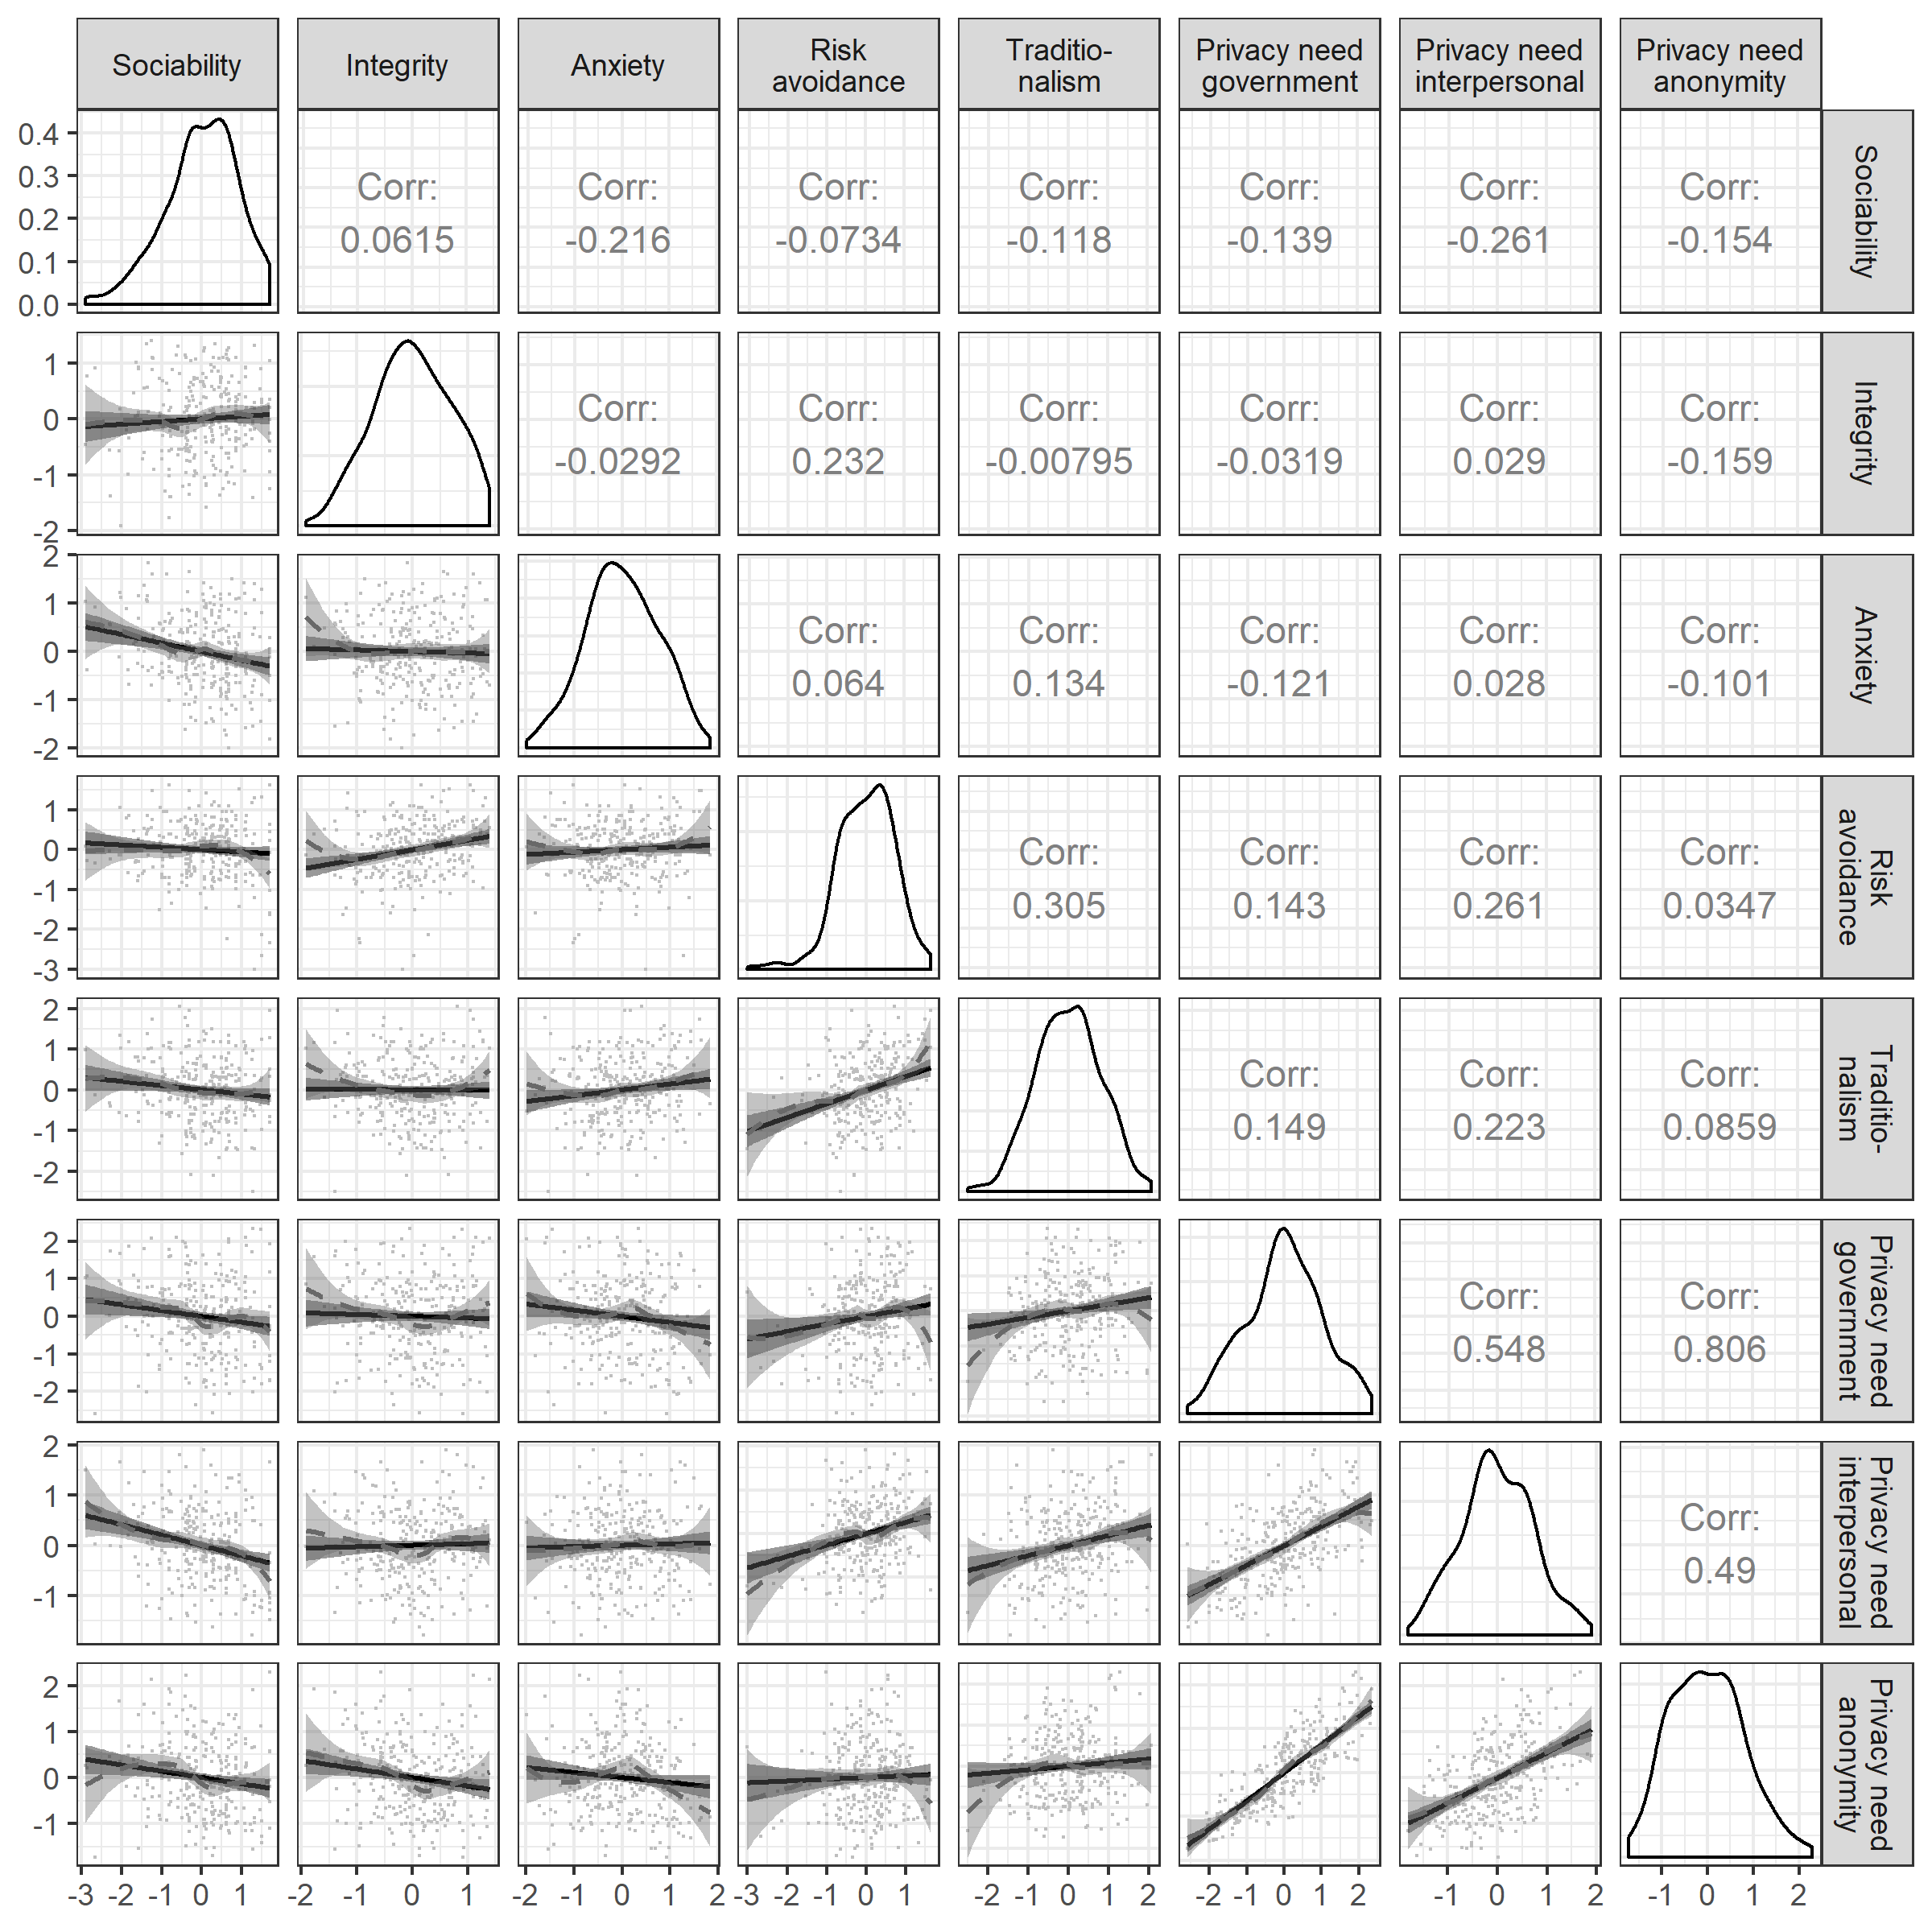
\includegraphics[width=.9\textwidth]{manuscript_files/figure-latex/bivar-fig-1} 

}

\caption{Results of the bivariate relations. Above diagonal: zero-order correlation matrix; diagonal: density plots for each variable; below diagonal: bivariate scatter plots for zero-order correlations. Solid regression lines represent linear regressions, dashed regression lines represent quadratic regressions. Calculated with the variables’ latent factor scores.}\label{fig:bivar-fig}
\end{figure}

\begin{figure}
\centering
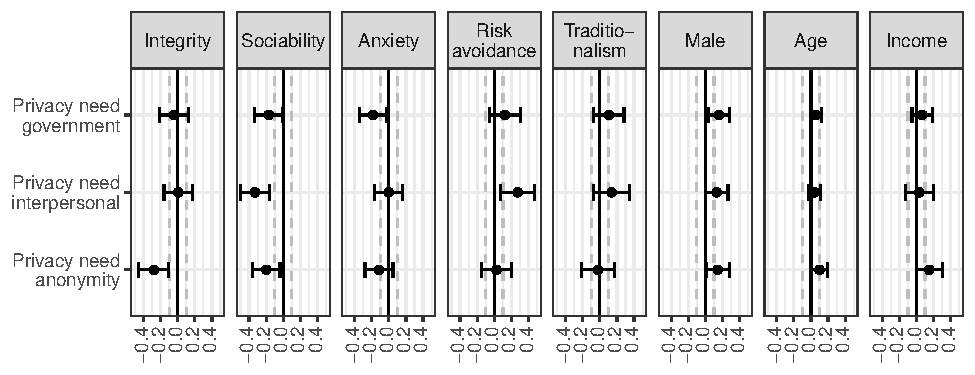
\includegraphics{manuscript_files/figure-latex/sem-fig-1.pdf}
\caption{\label{fig:sem-fig}Graphical overview of the results of Structural Equation Model. Shows the 95\% confidence intervals of standardized coefficients. Dashed lines indicate the SESOI of \textbar{}.10\textbar{}.}
\end{figure}

The bivariate correlations revealed that respondents who were more sociable than others also needed considerably less privacy from other people. In addition, they also needed slightly less privacy from the government and less anonymity. Also when analyzed in the multivariate structural regression model holding all other predictors constant, sociability was related to a reduced need for privacy on all three dimensions.

Next, both the bivariate and the SEM results showed that respondents who reported less integrity compared to others desired considerably more anonymity. No significant relations existed with the need for privacy from the government and the need for anonymity.

For anxiety, both analyses showed that respondents who indicated being more anxious indeed desired less privacy from the government. The effect size was small to moderate. Whereas the bivariate analyses revealed a small significant relation between anxiety and need for anonymity, this relation disappeared when analyzed in the SEM keeping all other predictors constant. No significant relationship with need for privacy from other people emerged.

Both analyses showed that respondents who reported being more risk avoidant than others desired considerably more privacy from other people. The bivariate analyses showed a small and positive association between risk avoidance and need for privacy from government surveillance, which ceased to exist in the SEM. No significant relation with need for anonymity was found.

\begin{table}[tbp]
\begin{center}
\begin{threeparttable}
\caption{\label{tab:sem-tab}Results of Structural Equation Model.}
\footnotesize{
\begin{tabular}{lrrrrr}
\toprule
Predictor & \multicolumn{1}{c}{b} & \multicolumn{1}{c}{ll} & \multicolumn{1}{c}{ul} & \multicolumn{1}{c}{beta} & \multicolumn{1}{c}{p}\\
\midrule
Privacy need government &  &  &  &  & \\
\ \ \ Sociability & -0.23 & -0.44 & -0.01 & -.17 & .037\\
\ \ \ Integrity & -0.07 & -0.37 & 0.22 & -.04 & .622\\
\ \ \ Anxiety & -0.31 & -0.58 & -0.03 & -.18 & .029\\
\ \ \ Traditionalism & 0.16 & -0.12 & 0.44 & .10 & .257\\
\ \ \ Risk avoidance & 0.20 & -0.10 & 0.51 & .12 & .197\\
\ \ \ Male & 0.38 & 0.08 & 0.68 & .16 & .012\\
\ \ \ Age & 0.03 & > -0.01 & 0.05 & .06 & .051\\
\ \ \ Income & 0.07 & -0.06 & 0.20 & .07 & .276\\
Privacy need interpersonal &  &  &  &  & \\
\ \ \ Sociability & -0.39 & -0.58 & -0.19 & -.33 & < .001\\
\ \ \ Integrity & 0.01 & -0.24 & 0.26 & .01 & .930\\
\ \ \ Anxiety & > -0.01 & -0.24 & 0.24 & > -.01 & .991\\
\ \ \ Traditionalism & 0.19 & -0.11 & 0.48 & .14 & .213\\
\ \ \ Risk avoidance & 0.40 & 0.12 & 0.67 & .27 & .005\\
\ \ \ Male & 0.28 & > -0.01 & 0.56 & .13 & .053\\
\ \ \ Age & 0.02 & -0.01 & 0.04 & .05 & .208\\
\ \ \ Income & 0.03 & -0.12 & 0.19 & .03 & .686\\
Privacy need anonymity &  &  &  &  & \\
\ \ \ Sociability & -0.22 & -0.40 & -0.04 & -.20 & .018\\
\ \ \ Integrity & -0.40 & -0.67 & -0.14 & -.28 & .003\\
\ \ \ Anxiety & -0.16 & -0.39 & 0.07 & -.11 & .167\\
\ \ \ Traditionalism & -0.03 & -0.29 & 0.23 & -.02 & .814\\
\ \ \ Risk avoidance & 0.04 & -0.21 & 0.28 & .03 & .770\\
\ \ \ Male & 0.29 & 0.01 & 0.58 & .14 & .041\\
\ \ \ Age & 0.03 & < 0.01 & 0.07 & .10 & .031\\
\ \ \ Income & 0.14 & -0.01 & 0.28 & .15 & .065\\
\bottomrule
\end{tabular}
}
\end{threeparttable}
\end{center}
\end{table}

Next, the bivariate analyses showed that respondents who scored higher on traditionalism also reported increased levels of need for privacy from government surveillance and other people. However, both relations disappeared in the SEM. No significant relation with need for anonymity was found.

Finally, regarding socio-demographic variables, the SEM showed that respondents who were older also desired slightly more anonymity. Male respondents desired more privacy from the government and more anonymity. Respondents with a higher income did not exhibit different levels of need for privacy.

Summarizing across the results, the predictors explained 12.04\% of the variance in need for privacy from the government, 28.27\% of the variance in need for privacy from other people, and 18.59\% of the variance in need for anonymity.

\hypertarget{discussion}{%
\section{Discussion}\label{discussion}}

This study analyzed the extent to which the need for privacy can be predicted and explained by personality traits. First, the results of the bivariate analyses showed that the need for privacy can be predicted surprisingly well by means of specific personality facets. Second, also when analyzed together in a structural regression model alongside additional socio-demographic variables, most personality variables remained significant, supporting the robustness of the relations.

Most prominently, we find that sociability was negatively related to all three dimensions of need for privacy. This does not come to much surprise as privacy captures the withdrawal from others and is hence already from a conceptual point of view closely related to sociability. Nonetheless, it is interesting to see that the relation is indeed thus proximal---especially in light of prior studies not having found a significant relation between extraversion and concern for privacy (Junglas et al., 2008), which are both related variables.

Next, and more controversial, our results also showed that the desire for anonymity is related substantially with measures of integrity. People who self-reported lower integrity desired more anonymity. Respondents who said, for example, that they would feel tempted to take things that do not belong to them were also more likely to avoid situations in which they were identifiable. This finding hence supports the logic behind the \enquote{nothing to hide} argument. It also follows Altman's privacy regulation theory (1976), which states that if exposure of information is risky it is likely that people will use more mechanisms to strengthen their social boundaries and increase their desired level of privacy. Importantly, however, integrity was not related to need for privacy from other people or to need for privacy from government surveillance, which hence limits the generalisability of the nothing-to-hide argument. In addition, note that the items measuring need for anonymity were very difficult (the mean was much lower compared to the other dimensions; see Table \ref{tab:psychometrics})---hence, the relationship between integrity and need for privacy might show only in very specific domains, for example, when it comes to avoiding places with video surveillance. In conclusion, the relation between integrity and need for privacy seems to be limited to certain aspects of need for privacy only. It should hence not be overly generalized.

Interestingly, the data showed that people who were more anxious were also more willing to accept government surveillance. This might be explained by the fact that governments are explicitly commissioned to help prevent crime or terrorist attacks, which are things more anxious people are more likely to dread.

People who were more risk averse desired more privacy from other people. Specifically, people who try to avoid risks are less inclined to share secrets with friends. This finding makes sense and can be aligned with prospect theory (Kahneman \& Tversky, 1979): The risks of a secret being publicly disclosed seem to outweigh the potential benefits of sharing it with confidants.

Finally, in the SEM no significant relations between need for privacy and traditionality were found. The results imply that independent from being more open to change or not, people desire the same level of privacy. Taken further, this finding might illustrate that a modern way of living does not necessarily imply a reduced need for privacy.

At a larger level, the results of this study highlight the importance of making differentiated claims on why people need privacy. Indeed, while the results suggest that some people might need anonymity because they may have something to hide, they also show that putting everyone who exhibits an increased need for privacy under suspicion is outright wrong. People who are less sociable, more risk averse, and less anxious are also more likely to need a bit more privacy. This implies that various personality-related aspects can predict need for privacy in different ways and for different reasons.

Another contribution this study makes to the privacy literature is that it is one of the first to explicitly distinguish different types of privacy needs. Specifically, we found that need for privacy consists of three separate dimensions, with factors measuring need for privacy from the government, need for privacy from other people, and need for anonymity. This factor solution is in line with privacy theory, which subsumes a vertical level (here, privacy from the government) and a horizontal level (here, privacy from other people) (e.g., Schwartz, 1968). The third dimension, need for anonymity, can be argued to exist on the diagonal, as one can be anonymous both from the government and from other people. The results of our study demonstrate the importance of differentiating these types of need for privacy, as relationships were not consistent across the various privacy needs and the five personality traits.

\hypertarget{limitations-and-future-research}{%
\subsection{Limitations and Future Research}\label{limitations-and-future-research}}

One can of course raise the question of whether it is possible or even socially desirable to measure a person's integrity. On the one hand, integrity implies absolute criteria in relation to social norms: Stealing is bad and forbidden, whereas helping is good and encouraged. On the other hand, integrity implies relative criteria: Whereas some cultures disapprove of lying whatever the context, others consider lying okay (for example, \enquote{white lies} in order to avoid hurting someone's feelings) (Altman, 1977). Thus, ranking behaviors, opinions, and character traits with regard to integrity presents a moral dilemma. As a result, throughout our study we have employed a conservative approach and understood and measured integrity as an explicit transgression of social norms that is strong and that most societies would arguably agree upon (for example, most societies would consider stealing as a sign of low integrity). Nonetheless, we recommend that future research should further elaborate on the general understanding of integrity as a theoretical concept. To date, there is not one overarching concept of integrity that incorporates all of the different aspects of this variable, and yet it would be valuable to examine how other aspects of integrity (e.g., authenticity, trustworthiness, or consistency) relate to need for privacy.

Worth nothing, integrity tests using self-reports have been shown to work surprisingly well, given that they can predict unwanted professional workplace behavior successfully (e.g., theft, drug and alcohol problems, or absenteeism) (Ones, Viswesvaran, \& Schmidt, 1993). In a meta-analysis with 665 correlation coefficients, self-reported integrity tests were associated with counterproductive behaviors with an average correlation coefficient of \emph{r} = .47 (Ones et al., 1993). Nonetheless, future research would evidently benefit from including behavioral manifestations of integrity, such as concrete cheating behaviors.

In what follows, we present some methodological points of criticism. Despite the fact that we used mostly well-established scales, confirmatory factor analyses showed that some of the original items had to be deleted to achieve adequate factorial validity. This resembles the finding by Hussey and Hughes (2018), who reported that several widely-used scales in psychological research actually do not show satisfactory factorial validity. By using bifactor models, however, it was possible to at least partially alleviate the problem. Next, in order to achieve sufficient factorial validity we needed to adapt the scales (for example by deleting items), which introduces problems of overfitting, which in turn potentially impedes the generalisability of the results (see, e.g., Yarkoni \& Westfall, 2017). However, by using bifactor models we explicitly tried to retain the largest possible number of items, which should render our results more robust. In addition, also when looking at the items individually (see OSM) one can see that the results are not overly dependent on inclusion of specific items. Another methodological improvement for future studies concerns the sample, which was comparatively small, leading to a reduced power to detect also small effects. Nonetheless, we are still confident that the results should be reliable, because we deliberately selected specific predictors that should exhibit at lest small to moderate relations with need for privacy (i.e., \emph{r} = .20). For small to moderate relations, the current study still had a convincing power of 91\%. Granted, when aiming to find also small effects (i.e., \emph{r} = .10) with a probability of 95\%, future studies would need to collect the answers of 1293 respondents (Cohen, 1992). Finally, generalisability is limited, as our sample was predominantly young, female, highly educated, and collected only in one single country.

Next, future research might consider analyzing predictors of privacy needs that are even more specified. For example, it is possible that people who hold dissenting political beliefs could also have a higher need for privacy from the government. In this study we focused mostly on escapist motives for why people desire privacy (e.g., sociability, risk aversion). Interestingly, Leary, Herbst, and McCrary (2003) showed that when predicting engagement in solitary activities, it is less preferable to measure how strongly people want to escape society (avoidance oriented), but rather how much they seek solitude (approach oriented). Hence, future studies might want to include predictors such as need for contemplation or trust (see, e.g., Metzger, 2004; Wheeless \& Grotz, 1977). Finally, it would be interesting to focus on need for privacy within different minority groups. For example, it seems plausible that people with a LGBT background might report needing more privacy from government (because it is potentially repressive or unfriendly toward LGBTs) or other people (especially weaker ties in their social networks who might not approve of their sexual identity).

\hypertarget{conclusion}{%
\subsection{Conclusion}\label{conclusion}}

In his novel \emph{The Circle}, Eggers (2013) describes a dystopian society in which people are gradually forfeiting their privacy. One after another becomes \enquote{transparent}: Carrying a small camera around the neck, people begin to broadcast their daily lives to the Internet. In the novel, this eventually causes a societal upheaval: \enquote{The pressure on those who hadn't gone transparent went from polite to oppressive. The question, from pundits and constituents, was obvious and loud: If you aren't transparent, what are you hiding?} (Eggers, 2013, p. 129).

The results of this study suggest that there might be some truth to the nothing-to-hide argument. However, the applicability seems to be limited to (very specific) aspects of anonymity (e.g., avoiding places with video surveillance or leaving one's ID at home). In general, the need for privacy seems to be related more closely to other aspects of personality.

\newpage

\hypertarget{references}{%
\section{References}\label{references}}

\begingroup
\setlength{\parindent}{-0.5in}
\setlength{\leftskip}{0.5in}

\hypertarget{refs}{}
\leavevmode\hypertarget{ref-Altman.1975}{}%
Altman, I. (1975). \emph{The environment and social behavior}. Monterey, CA: Brooks Cole.

\leavevmode\hypertarget{ref-Altman.1976}{}%
Altman, I. (1976). Privacy: A conceptual analysis. \emph{Environment and Behavior}, \emph{8}(1), 7--29. doi:\href{https://doi.org/10.1177/001391657600800102}{10.1177/001391657600800102}

\leavevmode\hypertarget{ref-Altman.1977}{}%
Altman, I. (1977). Privacy regulation: Culturally universal or culturally specific? \emph{Journal of Social Issues}, \emph{33}(3), 66--84. doi:\href{https://doi.org/10.1111/j.1540-4560.1977.tb01883.x}{10.1111/j.1540-4560.1977.tb01883.x}

\leavevmode\hypertarget{ref-R-papaja}{}%
Aust, F., \& Barth, M. (2018). \emph{papaja: Create APA manuscripts with R Markdown}. Retrieved from \url{https://github.com/crsh/papaja}

\leavevmode\hypertarget{ref-Bansal.2010}{}%
Bansal, G., Zahedi, F. M., \& Gefen, D. (2010). The impact of personal dispositions on information sensitivity, privacy concern and trust in disclosing health information online. \emph{Decision Support Systems}, \emph{49}(2), 138--150. doi:\href{https://doi.org/10.1016/j.dss.2010.01.010}{10.1016/j.dss.2010.01.010}

\leavevmode\hypertarget{ref-Bol.2018}{}%
Bol, N., Dienlin, T., Kruikemeier, S., Sax, M., Boerman, S. C., Strycharz, J., \ldots{} Vreese, C. H. de. (2018). Understanding the effects of personalization as a privacy calculus: Analyzing self-disclosure across health, news, and commerce contexts. \emph{Journal of Computer-Mediated Communication}, \emph{23}(6), 370--388. doi:\href{https://doi.org/10.1093/jcmc/zmy020}{10.1093/jcmc/zmy020}

\leavevmode\hypertarget{ref-boyd.2008c}{}%
boyd, danah m. (2008). \emph{Taken out of context. American teen sociality in networked publics: Doctoral dissertation}. Berkeley, CA: University of California.

\leavevmode\hypertarget{ref-Burgoon.1982}{}%
Burgoon, J. K. (1982). Privacy and communication. \emph{Annals of the International Communication Association}, \emph{1}, 206--249.

\leavevmode\hypertarget{ref-Buss.2001}{}%
Buss, A. H. (2001). \emph{Psychological dimensions of the self}. Thousand Oaks; Calif: Sage Publications.

\leavevmode\hypertarget{ref-R-pwr}{}%
Champely, S. (2018). \emph{Pwr: Basic functions for power analysis}. Retrieved from \url{https://CRAN.R-project.org/package=pwr}

\leavevmode\hypertarget{ref-Cohen.1992}{}%
Cohen, J. (1992). A power primer. \emph{Psychological Bulletin}, \emph{112}(1), 155--159. doi:\href{https://doi.org/10.1037/0033-2909.112.1.155}{10.1037/0033-2909.112.1.155}

\leavevmode\hypertarget{ref-Connelly.2006}{}%
Connelly, S., Lilienfeld, S. O., \& Schmeelk, K. M. (2006). Integrity tests and morality: Associations with ego development, moral reasoning, and psychopathic personality. \emph{International Journal of Selection and Assessment}, \emph{14}(1), 82--86. doi:\href{https://doi.org/10.1111/j.1468-2389.2006.00335.x}{10.1111/j.1468-2389.2006.00335.x}

\leavevmode\hypertarget{ref-Corcoran.1987}{}%
Corcoran, K. J., \& Rotter, J. B. (1987). Morality-conscience guilt scale as a predictor of ethical behavior in a cheating situation among college females. \emph{The Journal of General Psychology}, \emph{114}(2), 117--123. doi:\href{https://doi.org/10.1080/00221309.1987.9711061}{10.1080/00221309.1987.9711061}

\leavevmode\hypertarget{ref-Covey.1989}{}%
Covey, M. K., Saladin, S., \& Killen, P. J. (1989). Self-monitoring, surveillance, and incentive effects on cheating. \emph{The Journal of Social Psychology}, \emph{129}(5), 673--679. doi:\href{https://doi.org/10.1080/00224545.1989.9713784}{10.1080/00224545.1989.9713784}

\leavevmode\hypertarget{ref-DeCew.1997}{}%
DeCew, J. W. (1997). \emph{In pursuit of privacy: Law, ethics, and the rise of technology}. Ithaca, NY: Cornell Univ. Press.

\leavevmode\hypertarget{ref-Dienlin.2014}{}%
Dienlin, T. (2014). The privacy process model. In S. Garnett, S. Halft, M. Herz, \& J. M. Mönig (Eds.), \emph{Medien und Privatheit} (pp. 105--122). Passau, Germany: Karl Stutz.

\leavevmode\hypertarget{ref-Dienlin.2016a}{}%
Dienlin, T., \& Metzger, M. J. (2016). An extended privacy calculus model for SNSs---Analyzing self-disclosure and self-withdrawal in a representative U.S. sample. \emph{Journal of Computer-Mediated Communication}, \emph{21}(5), 368--383. doi:\href{https://doi.org/10.1111/jcc4.12163}{10.1111/jcc4.12163}

\leavevmode\hypertarget{ref-Donnellan.2008}{}%
Donnellan, M. B., \& Lucas, R. E. (2008). Age differences in the Big Five across the life span: Evidence from two national samples. \emph{Psychology and Aging}, \emph{23}(3), 558--566. doi:\href{https://doi.org/10.1037/a0012897}{10.1037/a0012897}

\leavevmode\hypertarget{ref-Eggers.2013}{}%
Eggers, D. (2013). \emph{The circle}. New York, NY: Knopf Publishing Group.

\leavevmode\hypertarget{ref-Fife.2012}{}%
Fife, E., \& Orjuel, J. (2012). The privacy calculus: Mobile apps and user perceptions of privacy and security. \emph{International Journal of Engineering Business Management}, \emph{4}, 1--10. doi:\href{https://doi.org/10.5772/51645}{10.5772/51645}

\leavevmode\hypertarget{ref-Granovetter.1973}{}%
Granovetter, M. S. (1973). The strength of weak ties. \emph{American Journal of Sociology}, \emph{78}(6), 1360--1380.

\leavevmode\hypertarget{ref-Greenwald.2013}{}%
Greenwald, G. (2013). NSA collecting phone records of millions of Verizon customers daily. \emph{The Guardian}. Retrieved from \url{www.theguardian.com}

\leavevmode\hypertarget{ref-Hussey.2018}{}%
Hussey, I., \& Hughes, S. (2018). Hidden invalidity among fifteen commonly used measures in social and personality psychology. doi:\href{https://doi.org/10.31234/osf.io/7rbfp}{10.31234/osf.io/7rbfp}

\leavevmode\hypertarget{ref-John.1999}{}%
John, O. P., \& Srivastava, S. (1999). The big five trait taxonomy: History, measurement, and theoretical perspectives. In L. A. Pervin \& O. P. John (Eds.), \emph{Handbook of personality} (pp. 102--138). New York, NY: Guilford Press.

\leavevmode\hypertarget{ref-Johnson.2010}{}%
Johnson, B. (2010). Privacy no longer a social norm, says Facebook founder. \emph{The Guardian}. Retrieved from \url{www.theguardian.com}

\leavevmode\hypertarget{ref-R-semTools}{}%
Jorgensen, D., T., Pornprasertmanit, S., Schoemann, M., A., \ldots{} Y. (2018). \emph{semTools: Useful tools for structural equation modeling}. Retrieved from \url{https://CRAN.R-project.org/package=semTools}

\leavevmode\hypertarget{ref-Junglas.2008}{}%
Junglas, I. A., Johnson, N. A., \& Spitzmüller, C. (2008). Personality traits and concern for privacy: an empirical study in the context of location-based services. \emph{European Journal of Information Systems}, \emph{17}(4), 387--402. doi:\href{https://doi.org/10.1057/ejis.2008.29}{10.1057/ejis.2008.29}

\leavevmode\hypertarget{ref-Kahneman.1979}{}%
Kahneman, D., \& Tversky, A. (1979). Prospect theory: An analysis of decision under risk. \emph{Econometrica}, \emph{47}(2), 263. doi:\href{https://doi.org/10.2307/1914185}{10.2307/1914185}

\leavevmode\hypertarget{ref-Kline.2016}{}%
Kline, R. B. (2016). \emph{Principles and practice of structural equation modeling} (4th ed.). New York, NY: The Guilford Press.

\leavevmode\hypertarget{ref-R-MVN}{}%
Korkmaz, S., Goksuluk, D., \& Zararsiz, G. (2014). MVN: An r package for assessing multivariate normality. \emph{The R Journal}, \emph{6}(2), 151--162. Retrieved from \url{https://journal.r-project.org/archive/2014-2/korkmaz-goksuluk-zararsiz.pdf}

\leavevmode\hypertarget{ref-Lakens.2018}{}%
Lakens, D., Scheel, A. M., \& Isager, P. M. (2018). Equivalence testing for psychological research: A tutorial. \emph{Advances in Methods and Practices in Psychological Science}, \emph{1}(2), 259--269. doi:\href{https://doi.org/10.1177/2515245918770963}{10.1177/2515245918770963}

\leavevmode\hypertarget{ref-Leary.2003}{}%
Leary, M. R., Herbst, K. C., \& McCrary, F. (2003). Finding pleasure in solitary activities: Desire for aloneness or disinterest in social contact? \emph{Personality and Individual Differences}, \emph{35}(1), 59--68. doi:\href{https://doi.org/10.1016/S0191-8869(02)00141-1}{10.1016/S0191-8869(02)00141-1}

\leavevmode\hypertarget{ref-Masur.2018}{}%
Masur, P. K. (2018). \emph{Situational privacy and self-disclosure: Communication processes in online environments}. Cham, Switzerland: Springer.

\leavevmode\hypertarget{ref-Meijer.2016}{}%
Meijer, R. R., Niessen, A. S. M., \& Tendeiro, J. N. (2016). A practical guide to check the consistency of item response patterns in clinical research through person-fit statistics: Examples and a computer Program. \emph{Assessment}, \emph{23}(1), 52--62. doi:\href{https://doi.org/10.1177/1073191115577800}{10.1177/1073191115577800}

\leavevmode\hypertarget{ref-Metzger.2004}{}%
Metzger, M. J. (2004). Privacy, trust, and disclosure: Exploring barriers to electronic commerce. \emph{Journal of Computer-Mediated Communication}, \emph{9}(4). doi:\href{https://doi.org/10.1111/j.1083-6101.2004.tb00292.x}{10.1111/j.1083-6101.2004.tb00292.x}

\leavevmode\hypertarget{ref-Morton.2013}{}%
Morton, A. (2013). Measuring inherent privacy concern and desire for privacy - A pilot survey study of an instrument to measure dispositional privacy concern. In \emph{International Conference on Social Computing (SocialCom)} (pp. 468--477). doi:\href{https://doi.org/10.1109/SocialCom.2013.73}{10.1109/SocialCom.2013.73}

\leavevmode\hypertarget{ref-Nissenbaum.2010}{}%
Nissenbaum, H. (2010). \emph{Privacy in context: Technology, policy, and the integrity of social life}. Stanford, CA: Stanford University Press.

\leavevmode\hypertarget{ref-Omarzu.2000}{}%
Omarzu, J. (2000). A disclosure decision model: Determining how and when individuals will self-disclose. \emph{Personality and Social Psychology Review}, \emph{4}(2), 174--185. doi:\href{https://doi.org/10.1207/S15327957PSPR0402_5}{10.1207/S15327957PSPR0402\_5}

\leavevmode\hypertarget{ref-Ones.1993}{}%
Ones, D. S., Viswesvaran, C., \& Schmidt, F. L. (1993). Comprehensive meta-analysis of integrity test validities: Findings and implications for personnel selection and theories of job performance. \emph{Journal of Applied Psychology}, \emph{78}(4), 679--703. doi:\href{https://doi.org/10.1037/0021-9010.78.4.679}{10.1037/0021-9010.78.4.679}

\leavevmode\hypertarget{ref-Park.2015}{}%
Park, Y. J. (2015). Do men and women differ in privacy? Gendered privacy and (in)equality in the Internet. \emph{Computers in Human Behavior}, \emph{50}, 252--258. doi:\href{https://doi.org/10.1016/j.chb.2015.04.011}{10.1016/j.chb.2015.04.011}

\leavevmode\hypertarget{ref-Paunonen.2002}{}%
Paunonen, S. V. (2002). Design and construction of the Supernumerary Personality Inventory. London, Canada: University of Western Ontario.

\leavevmode\hypertarget{ref-Paunonen.2001}{}%
Paunonen, S. V., \& Ashton, M. C. (2001). Big Five factors and facets and the prediction of behavior. \emph{Journal of Personality and Social Psychology}, \emph{81}(3), 524--539. doi:\href{https://doi.org/10.1037/0022-3514.81.3.524}{10.1037/0022-3514.81.3.524}

\leavevmode\hypertarget{ref-Pedersen.1979}{}%
Pedersen, D. M. (1979). Dimensions of privacy. \emph{Perceptual and Motor Skills}, \emph{48}(3), 1291--1297. doi:\href{https://doi.org/10.2466/pms.1979.48.3c.1291}{10.2466/pms.1979.48.3c.1291}

\leavevmode\hypertarget{ref-Pedersen.1982}{}%
Pedersen, D. M. (1982). Personality correlates of privacy. \emph{The Journal of Psychology}, \emph{112}(1), 11--14. doi:\href{https://doi.org/10.1080/00223980.1982.9923528}{10.1080/00223980.1982.9923528}

\leavevmode\hypertarget{ref-Petronio.2010}{}%
Petronio, S. (2010). Communication privacy management theory: What do we know about family privacy regulation? \emph{Journal of Family Theory \& Review}, \emph{2}(3), 175--196. doi:\href{https://doi.org/10.1111/j.1756-2589.2010.00052.x}{10.1111/j.1756-2589.2010.00052.x}

\leavevmode\hypertarget{ref-PewResearchCenter.2015c}{}%
Pew Research Center. (2015). Beyond distrust: How Americans view their government. Retrieved from \url{http://www.people-press.org/2015/11/23/beyond-distrust-how-americans-view-their-government/}

\leavevmode\hypertarget{ref-PewResearchCenter.2017}{}%
Pew Research Center. (2017). Public trust in government: 1958-2017. Retrieved from \url{http://www.people-press.org/2017/12/14/public-trust-in-government-1958-2017/}

\leavevmode\hypertarget{ref-R-base}{}%
R Core Team. (2018). \emph{R: A language and environment for statistical computing}. Vienna, Austria: R Foundation for Statistical Computing. Retrieved from \url{https://www.R-project.org/}

\leavevmode\hypertarget{ref-R-psych}{}%
Revelle, W. (2018). \emph{Psych: Procedures for psychological, psychometric, and personality research}. Evanston, Illinois: Northwestern University. Retrieved from \url{https://CRAN.R-project.org/package=psych}

\leavevmode\hypertarget{ref-R-lavaan}{}%
Rosseel, Y. (2012). lavaan: An R package for structural equation modeling. \emph{Journal of Statistical Software}, \emph{48}(2), 1--36. Retrieved from \url{http://www.jstatsoft.org/v48/i02/}

\leavevmode\hypertarget{ref-R-GGally}{}%
Schloerke, B., Crowley, J., Cook, D., Briatte, F., Marbach, M., Thoen, E., \ldots{} Larmarange, J. (2018). \emph{GGally: Extension to 'ggplot2'}. Retrieved from \url{https://CRAN.R-project.org/package=GGally}

\leavevmode\hypertarget{ref-Schwartz.1968}{}%
Schwartz, B. (1968). The social psychology of privacy. \emph{American Journal of Sociology}, \emph{73}(6), 741--752.

\leavevmode\hypertarget{ref-Sevignani.2016}{}%
Sevignani, S. (2016). \emph{Privacy and capitalism in the age of social media}. New York; London: Routledge Taylor \& Francis Group.

\leavevmode\hypertarget{ref-Sheldon.2004}{}%
Sheldon, K. M. (2004). Integrity {[}authenticity, honesty{]}. In C. Peterson \& Seligman, M. E. P. (Eds.), \emph{Character strengths and virtues: A handbook and classification} (pp. 249--271). Oxford, UK: Oxford University Press.

\leavevmode\hypertarget{ref-Solove.2007}{}%
Solove, D. J. (2007). 'I've got nothing to hide' and other misunderstandings of privacy. \emph{San Diego Law Review}, \emph{44}, 745--772.

\leavevmode\hypertarget{ref-Stone.1986}{}%
Stone, D. L. (1986). Relationship between introversion/extraversion, values regarding control over information, and perceptions of invasion of privacy. \emph{Perceptual and Motor Skills}, \emph{62}(2), 371--376. doi:\href{https://doi.org/10.2466/pms.1986.62.2.371}{10.2466/pms.1986.62.2.371}

\leavevmode\hypertarget{ref-R-PerFit}{}%
Tendeiro, J. N., Meijer, R. R., \& Niessen, A. S. M. (2016). PerFit: An R package for person-fit analysis in IRT. \emph{Journal of Statistical Software}, \emph{74}(5), 1--27. doi:\href{https://doi.org/10.18637/jss.v074.i05}{10.18637/jss.v074.i05}

\leavevmode\hypertarget{ref-Tifferet.2019}{}%
Tifferet, S. (2019). Gender differences in privacy tendencies on social network sites: A meta-analysis. \emph{Computers in Human Behavior}, \emph{93}, 1--12. doi:\href{https://doi.org/10.1016/j.chb.2018.11.046}{10.1016/j.chb.2018.11.046}

\leavevmode\hypertarget{ref-Trepte.2013a}{}%
Trepte, S., Dienlin, T., \& Reinecke, L. (2013). Privacy, self-disclosure, social support, and social network site use. Research report of a three-year panel study. Retrieved from \url{http://opus.uni-hohenheim.de/volltexte/2013/889/}

\leavevmode\hypertarget{ref-Trepte.2017d}{}%
Trepte, S., \& Masur, P. K. (2017). Need for privacy. In V. Zeigler-Hill \& T. K. Shackelford (Eds.), \emph{Encyclopedia of Personality and Individual Differences} (Vol. 94, pp. 1--4). Cham: Springer International Publishing. doi:\href{https://doi.org/10.1007/978-3-319-28099-8_540-1}{10.1007/978-3-319-28099-8\_540-1}

\leavevmode\hypertarget{ref-R-mice}{}%
van Buuren, S., \& Groothuis-Oudshoorn, K. (2011). mice: Multivariate imputation by chained equations in r. \emph{Journal of Statistical Software}, \emph{45}(3), 1--67. Retrieved from \url{https://www.jstatsoft.org/v45/i03/}

\leavevmode\hypertarget{ref-Weinberger.2017b}{}%
Weinberger, M., Zhitomirsky-Geffet, M., \& Bouhnik, D. (2017). Sex differences in attitudes towards online privacy and anonymity among Israeli students with different technical backgrounds, \emph{22}(4). Retrieved from \url{http://InformationR.net/ir/22-4/paper777.html}

\leavevmode\hypertarget{ref-Westin.1967}{}%
Westin, A. F. (1967). \emph{Privacy and freedom}. New York, NY: Atheneum.

\leavevmode\hypertarget{ref-Wheeless.1977}{}%
Wheeless, L. R., \& Grotz, J. (1977). The measurement of trust and its relationship to self-disclosure. \emph{Human Communication Research}, \emph{3}(3), 250--257. doi:\href{https://doi.org/10.1111/j.1468-2958.1977.tb00523.x}{10.1111/j.1468-2958.1977.tb00523.x}

\leavevmode\hypertarget{ref-R-ggplot2}{}%
Wickham, H. (2016). \emph{Ggplot2: Elegant graphics for data analysis}. Springer-Verlag New York. Retrieved from \url{http://ggplot2.org}

\leavevmode\hypertarget{ref-R-tidyverse}{}%
Wickham, H. (2017). \emph{Tidyverse: Easily install and load the 'tidyverse'}. Retrieved from \url{https://CRAN.R-project.org/package=tidyverse}

\leavevmode\hypertarget{ref-R-knitr}{}%
Xie, Y. (2015). \emph{Dynamic documents with R and knitr} (2nd ed.). Boca Raton, Florida: Chapman; Hall/CRC. Retrieved from \url{https://yihui.name/knitr/}

\leavevmode\hypertarget{ref-Yarkoni.2017}{}%
Yarkoni, T., \& Westfall, J. (2017). Choosing prediction over explanation in psychology: Lessons from machine learning. \emph{Perspectives on psychological science : a journal of the Association for Psychological Science}, \emph{12}(6), 1100--1122. doi:\href{https://doi.org/10.1177/1745691617693393}{10.1177/1745691617693393}

\endgroup

\newpage

\hypertarget{contributions}{%
\section{Contributions}\label{contributions}}

\begin{itemize}
\tightlist
\item
  Contributed to conception and design: TD, MM
\item
  Contributed to acquisition of data: MM, TD
\item
  Contributed to analysis and interpretation of data: TD, MM
\item
  Drafted and/or revised the article: TD, MM
\item
  Approved the submitted version for publication: TD, MM
\end{itemize}

\hypertarget{funding-information}{%
\section{Funding Information}\label{funding-information}}

During the conception and data collection of the study, TD was funded by The German Academic Scholarship Foundation (German: Studienstiftung des deutschen Volkes), which financially supported TD's research stay at UCSB. During the writing of the article, TD was funded by the Volkswagen Foundation (German: Volkswagenstiftung), grant \enquote{Transformations of Privacy}.

MM is funded by a regular and tenured full professorship at UCSB.

\hypertarget{competing-interests}{%
\section{Competing Interests}\label{competing-interests}}

We declare no competing interests.

\hypertarget{data-accessibility-statement}{%
\section{Data Accessibility Statement}\label{data-accessibility-statement}}

All the stimuli, presentation materials, participant data, analysis scripts, and a reproducible version of the manuscript can be found on this paper's project page on the open science framework (\url{https://osf.io/7ncpk/?view_only=38283fd9262646378e4ba1e19c9d707f}). In addition, we invite everyone to suggest changes and improvements to the manuscript via our github (\url{https://github.com/tdienlin/need_for_privacy/tree/master}).


\end{document}
